\documentclass[a4paper,12pt,oneside,final]{report}
%\usepackage{geometry}                % See geometry.pdf to learn the layout options. There are lots.
%\geometry{landscape}                % Activate for for rotated page geometry
%\usepackage[parfill]{parskip}    % Activate to begin paragraphs with an empty line rather than an indent
\usepackage{graphicx}
% \usepackage{amssymb}
\usepackage{epstopdf}
\usepackage[utf8]{inputenc}
\usepackage{titlesec}
\usepackage[titletoc]{appendix}
\titleformat{\chapter}[hang]{\bf\Huge}{\thechapter}{1cm}{}

\pagestyle{plain}
% -------------------- this stuff for code --------------------

\usepackage{anysize}
\marginsize{30mm}{30mm}{20mm}{20mm}

\newenvironment{formal}{%
  \def\FrameCommand{%
    \hspace{1pt}%
    {\color{blue}\vrule width 2pt}%
    {\color{formalshade}\vrule width 4pt}%
    \colorbox{formalshade}%
  }%
  \MakeFramed{\advance\hsize-\width\FrameRestore}%
  \noindent\hspace{-4.55pt}% disable indenting first paragraph
  \begin{adjustwidth}{}{7pt}%
  \vspace{2pt}\vspace{2pt}%
}
{%
  \vspace{2pt}\end{adjustwidth}\endMakeFramed%
}

\newenvironment{changemargin}[2]{\begin{list}{}{%
\setlength{\topsep}{0pt}%
\setlength{\leftmargin}{0pt}%
\setlength{\rightmargin}{0pt}%
\setlength{\listparindent}{\parindent}%
\setlength{\itemindent}{\parindent}%
\setlength{\parsep}{0pt plus 1pt}%
\addtolength{\leftmargin}{#1}%
\addtolength{\rightmargin}{#2}%
}\item }{\end{list}}

\usepackage{color}
\usepackage{dsfont}
\usepackage[bitstream-charter]{mathdesign}
\usepackage[scaled]{helvet}
\usepackage{inconsolata}


\definecolor{colKeys}{rgb}{0,0,0.9} 
\definecolor{colIdentifier}{rgb}{0,0,0} 
\definecolor{colString}{rgb}{0.7,0,0} 
\definecolor{colComments}{rgb}{0,0.6,0} 
\usepackage{listings}
\lstset{
  stringstyle=\color{colString},
  keywordstyle=\color{colKeys},
  identifierstyle=\color{colIdentifier},
  commentstyle=\color{colComments},
  numbers=left,
  tabsize=4,
  frame=single,
  breaklines=true,
  basicstyle=\small\ttfamily,
  numberstyle=\tiny\ttfamily,
  framexleftmargin=0mm,
  xleftmargin=7mm,
  xrightmargin=7mm,
  frameround={tttt},
  captionpos=b
}

%% Headers and footers
\usepackage{fancyhdr}
\usepackage[section]{placeins}
\pagestyle{fancy}
\fancyhf{}
\addtolength{\headwidth}{30pt}
\addtolength{\headwidth}{30pt}
\renewcommand{\headrulewidth}{0.4pt} % thickness of the header line
\renewcommand{\footrulewidth}{0.4pt} % thickness of the footer line
\renewcommand{\chaptermark}[1]{\markboth{#1}{#1}} % chapter name
\renewcommand{\sectionmark}[1]{\markright{\thesection\ #1}}  % section name
\lhead[\fancyplain{}{\bf\thepage}]{\fancyplain{}{\bf\rightmark}} % display header
\rhead[\fancyplain{}{\bf\leftmark}]{\fancyplain{}{}} % display header
\fancyfoot[C]{\bf\thepage} % display footer (page number)
\fancyfoot[R]{\bf\today} % display footer (date)
\fancypagestyle{plain}{ 
	\fancyhead{} \renewcommand{\headrulewidth}{0pt}
}
\newcommand{\clearemptydoublepage}{\newpage{\pagestyle{plain}\cleardoublepage}}

\usepackage[T1]{fontenc}
\usepackage{enumerate}
\usepackage{afterpage,lastpage,fancyhdr}
\usepackage[includeheadfoot,margin=2.5cm]{geometry}
\geometry{letterpaper}                   % ... or a4paper or a5paper or ... 

% -------------------- end of code stuff --------------------



\DeclareGraphicsRule{.tif}{png}{.png}{`convert #1 `dirname #1`/`basename #1 .tif`.png}

\makeatletter \def\thickhrulefill{\leavevmode \leaders \hrule height 1pt\hfill
\kern \z@} \renewcommand{\maketitle}{
    \begin{titlepage}
    \let\footnotesize\small \let\footnoterule\relax \parindent \z@ \reset@font
    \null\vfil
    \vspace{-20mm}
    \begin{center}
    {\small \scshape Imperial College London}
    \end{center}
    \vspace{0.5cm}
	\begin{minipage}{\textwidth}
		\vspace{1cm}
		%\noindent\rule[0ex]{\textwidth}{4pt} \\
		%\flushright
		\center
		\@title
		\\ \vspace{4mm}
		%\noindent\rule[0ex]{\textwidth}{4pt} \\
	\end{minipage}
	\vspace{2cm}
	\begin{center}
		
\includegraphics[width=70mm,]{logo_imperial_college_london.png}
	\end{center}
	\vspace{5.4cm}
	\vspace{\stretch{1}}
	\begin{minipage}{\textwidth}
		\flushright
		{\bfseries}
		\vspace{7mm}
		\center
		\@author\\
	\end{minipage}
	\vspace{20mm}
		\flushleft
		{\bfseries}
		{\small \scshape \@date }
		\vspace{0.1cm}
		\rule{\linewidth}{.5pt}
  \end{titlepage}
  \setcounter{footnote}{1}
  \setcounter{page}{2}
}


\author{Paul Gribelyuk (pg1312, a5)}
\makeatother
\title{\Huge \#DOC417 - Advanced Computer Graphics Coursework 1}
\date{\today}

\begin{document}
\maketitle
% \tableofcontents
\listoffigures
\chapter{Generating HDR Images}
\paragraph{}
This part asked to produce an HDR image with the 7 included low-dynamic-range files according to the following formula:
$$
f(x,y) = \exp\left\{\frac{\sum_i w(Z_i(x,y))\log\left(\frac{Z_i(x,y)}{\Delta t_i}\right)}{\sum_i w(Z_i(x,y)}\right\}
$$
\paragraph{}
Since we assumed a linear response function $f$, we are able to use this simplifying assumption in the calculation.  The assignment asked to implement a re-weighting function which has the effect of giving greater weight to pixels of images with a middle-of-the-range value.  The one I used was:
$$
w(z) = \frac{1}{2} + \frac{1}{2}\cdot\sin\left(2\pi\left(z - \frac{1}{4})\right)\right)
$$
 Since the relative exposure is inversely proportional to the intensity of the pixel being computed, this has the effect of dampening the end-result to a very dark exposure, seen here:
\begin{figure}[!h]
\begin{changemargin}{-50mm}{-50mm}
\center
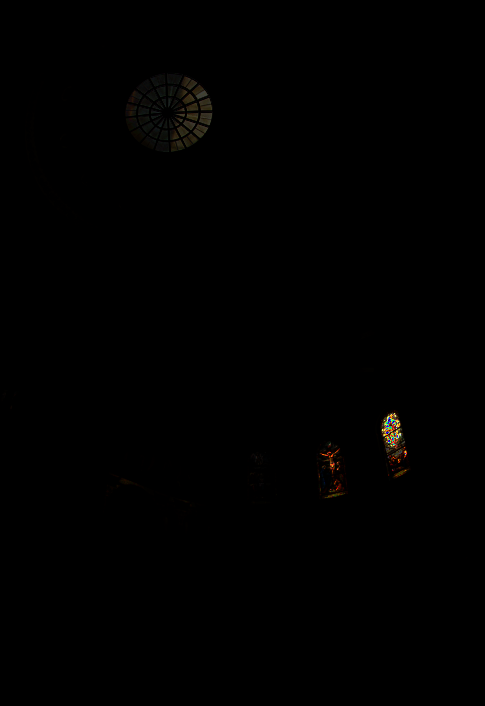
\includegraphics[scale=0.3]{memorial_hdr.png}
\caption{HDR Image before further processing}
\end{changemargin}
\end{figure}

To fix this, I stretched the pixel values so that the minimum (overall, not per channel) value was at zero and the maximum was at one and applied a 5000 brightness scaling (keeping maximum at 1).  This is seen here:
\begin{figure}[!h]
\begin{changemargin}{-50mm}{-50mm}
\center
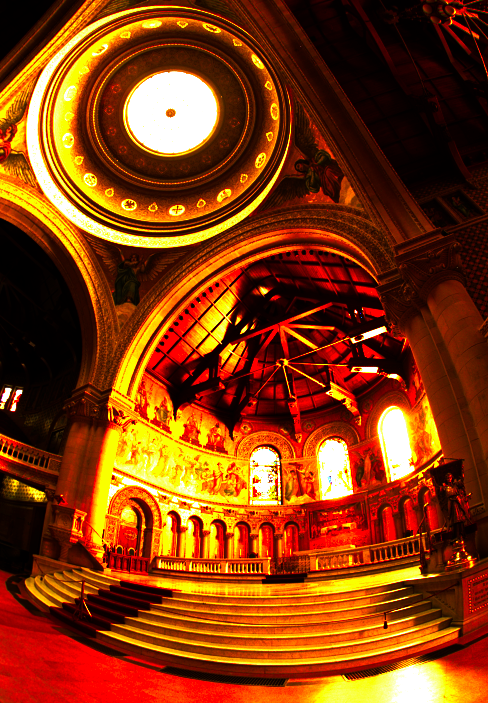
\includegraphics[scale=0.35]{memorial_hdr_stretched.png}
\caption{HDR Image after tone mapping and brightening}
\end{changemargin}
\end{figure}

I also applied a few different gamma settings to make the image friendlier to the human eye:
\begin{figure}[!h]
\begin{changemargin}{-50mm}{-50mm}
\center
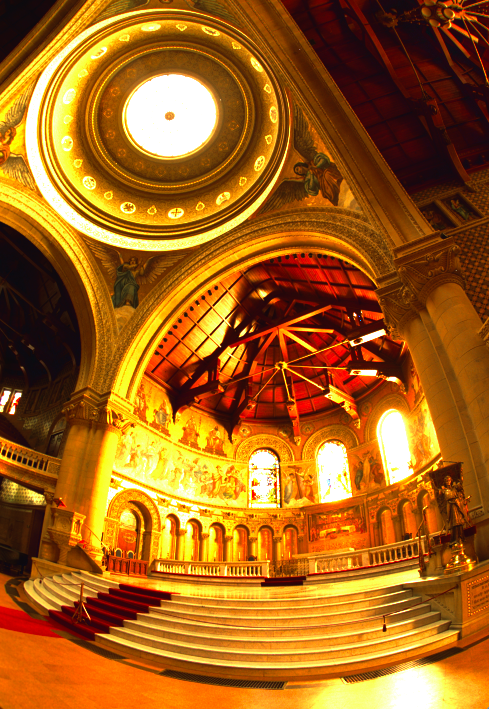
\includegraphics[scale=0.35]{memorial_gamma_18.png}
\caption{HDR Image with Gamma adjustment of 1.8}
\end{changemargin}
\end{figure}

\begin{figure}[!h]
\begin{changemargin}{-50mm}{-50mm}
\center
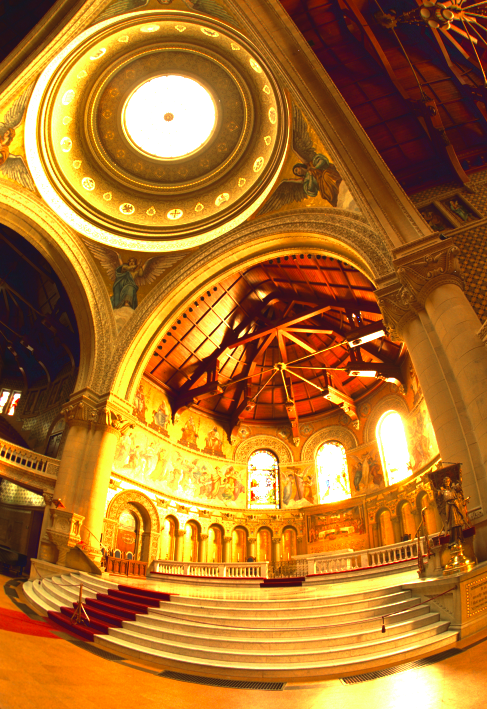
\includegraphics[scale=0.35]{memorial_gamma_22.png}
\caption{HDR Image with Gamma adjustment of 2.2}
\end{changemargin}
\end{figure}

\begin{figure}[!h]
\begin{changemargin}{-50mm}{-50mm}
\center
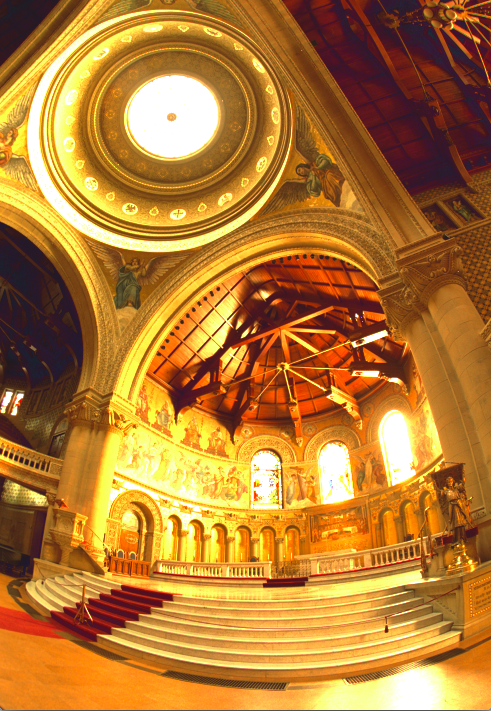
\includegraphics[scale=0.35]{memorial_gamma_25.png}
\caption{HDR Image with Gamma adjustment of 2.5}
\end{changemargin}
\end{figure}

Although it is pretty clear that 2.2 is the optimal gamma adjustment, and has been widely applied in graphics software in industry, the Mac OS X operating system used a gamma of 1.8 up until the 10.6 version release in 2009.  I also noticed that different brightness adjustments (stops) were better with different gamma settings, i.e. a higher gamma allowed for a lower brightness adjustment, and vice versa, although at extremes, this relationship produced bad images, highlighting the tradeoff between these two settings.

\FloatBarrier

\chapter{Implementing Image-Based Lighting}
\paragraph{}
This part of the assignment asked to first visualize the reflectance vectors on a sphere in a 511 by 511 image, with the three different channels representing the three coordinates.  The general reflectance formula is:
$$
\mathbf{r} = 2(\mathbf{n}\cdot\mathbf{v})\mathbf{n} - \mathbf{v}
$$
with the normal $\mathbf{n}$ being defined as:
\begin{eqnarray}
x = \frac{2j}{d} - 1\\
y = 1 - \frac{2i}{d} \\
z = \sqrt{1 - x^2 - y^2}
\end{eqnarray}
with $i$ and $j$ representing the height and width pixel indices, respectively, and $d$ being the number of pixels for the length of the diameter of the sphere being constructed.

Thus, since, Blue is the third channel, it should appear close to the center of the sphere, since, there, rays are being reflected back at the camera, in the positive $z$ direction.  Indeed, we see this relationship in the image below:
\begin{figure}[!h]
\begin{changemargin}{-50mm}{-50mm}
\center
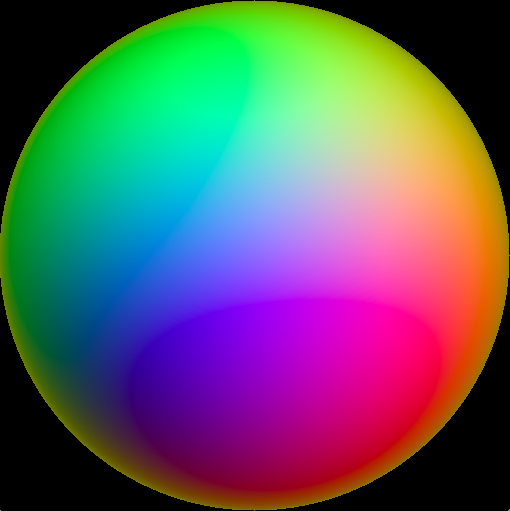
\includegraphics[scale=0.5]{reflectance_map.png}
\caption{Reflection Map on a Sphere}
\end{changemargin}
\end{figure}

\paragraph{}
The next, and last part of the assignment is to map a lat-long map of a scene onto a mirrored ball.  For this, it is beneficial to use the reflectance vectors already consructed in the previous part of the assignment, and to transform them to polar coordinates $(\theta, \phi)$ (since radius is one) with the following formulae:
\begin{eqnarray}
\theta &=& \arccos(r[1]) \\
\phi &=& \arctan\left(\frac{r[0]}{r[2]}\right)\\
\end{eqnarray}
These variables represent where on the lat-long map the pixel is to be found corresponding to the ray $\mathbf{r}$ and its unique point on the sphere.  Unfortunately, my code had a small mistake I could not find, but the result is here:
\begin{figure}[!h]
\begin{changemargin}{-50mm}{-50mm}
\center
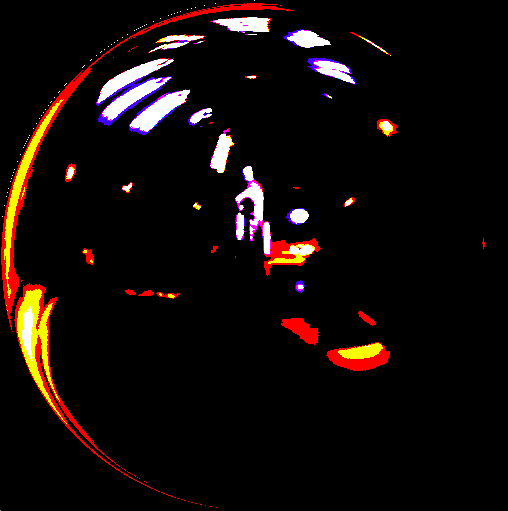
\includegraphics[scale=0.4]{grace_sphere.png}
\caption{Mapping the Grace Cathedral Lat-Long Environment Map onto a Sphere}
\end{changemargin}
\end{figure}


\paragraph{}
In conclusion, I have written everything in C, code is available upon demand, and the corresponding PFM images are included in the zip file.
\end{document}  
